\documentclass{article}
\usepackage{authblk}
\usepackage{hyperref}
\usepackage{graphicx}
\begin{document}
% Title of paper
\title{Prediction of Aging by Gene Expression}

% List of authors, with corresponding author marked by asterisk
\author{F. William Townes$^{1}$, Jeffrey W. Miller$^{1}$}%\\[4pt]
% Author addresses
\affil{\footnotesize $^{1}$Department of Biostatistics, Harvard T.H. Chan School of Public Health, Boston, MA \\%}[2pt]
% E-mail address for correspondence
\normalsize {ftownes@g.harvard.edu, jwmiller@hsph.harvard.edu}
}
\maketitle

\newpage
\begin{abstract}
Return
\end{abstract}

\section{Introduction}
Identifying the genetic and molecular basis for aging is a long standing goal in medical science. Many studies have investigated whether individual genes are pro-aging or anti-aging on a case by case basis. Typically, a direct intervention such as a knockout or chemical perturbation is applied to a small number of genes in a model organism such as yeast or C. elegans followed by quantification of lifespan. These experiments are capable of identifying causal relationships, but are slow and expensive. In order to prioritize which genes to examine next and speed up the process, recent studies have used annotations like the Gene Ontology (GO) to computationally predict the effect of any gene on aging. A recent survey of such efforts is provided by \cite{fabris_review_2017}. Recent studies suffer from several limitations. First, annotations like GO may be biased by the scope of the existing literature. Second, there is no consistency between studies in algorithms, feature sets, or predictive outcome, making it difficult to compare results. Finally, most recent studies do not report a predictive score on a held-out test dataset, leading to overestimating the performance of the algorithms.

We address these gaps in the computational aging literature by systematically assessing the performance of common machine learning algorithms on predicting pro- versus anti- aging status of genes in yeast and C. elegans. We compare the efficacy of GO terms as predictors against gene expression profiles from the ARCHS4 database. We use a consistent target outcome in all comparisons, drawn from the GenAge database. Finally, we provide predictions for top candidate genes that were not annotated in GenAge to suggest directions for future experimental studies.

\section{Methods}

Binary pro/anti aging annotations were accessed from the GenAge model organisms database \url{http://genomics.senescence.info/genes}. We subset on yeast and worm and excluded ambiguous annotations. GO annotations for all genes were downloaded from BioMart ENSEMBL database using Bioconductor package biomaRt. For both species, gene expression (RNA-Seq read counts) data were obtained from the ARCHS4 database \url{https://amp.pharm.mssm.edu/archs4/archs4zoo.html}. Additionally, for yeast only, microarray expression measurements were acquired from Deleteome \url{http://deleteome.holstegelab.nl}. Finally, for worm only, gene expression from the single cell RNA-Seq Worm Cell Atlas \url{http://atlas.gs.washington.edu/worm-rna} was utilized. Unique molecular identifier (UMI) counts were summed across all cells within the same tissue.

All gene expression measurements were normalized to account for sample-specific biases. Specifically, the Deleteome data were already normalized, the ARCHS4 read counts were converted to transcripts-per-million (TPM), and the worm atlas UMIs to counts-per-million (CPM). The normalized counts were then log transformed with a pseudocount of one. For deleteome, genes that were variable in controls and non-responsive mutants were excluded. For each species, the data were subset by taking the intersection of genes with no missing values across all feature types (GO and two types of gene expression), resulting in 703 worm genes (246 pro, 457 anti aging) and 368 yeast genes (46 pro, 322 anti aging). Features with no variation across the included genes were discarded. For yeast, the number of retained features was 3268, 700, and 1390 for ARCHS4, deleteome, and GO terms respectively. For worms, the number of features was 2935, 270, and 2051 for ARCHS4, cell atlas, and GO terms respectively. All gene expression features were centered and scaled to have mean zero and standard deviation 0.5, while binary features (GO) were left as-is. The five final feature sets for each species were ARCHS4 alone, GO alone, gene expression alone (deleteome for yeast or worm cell atlas), GO combined with ARCHS4, and GO combined with gene expression.

To assess predictive performance of different combinations of feature sets on pro versus anti aging status of each gene, each dataset was split into 5 cross-validation (CV) folds. Within each fold, machine learning classifiers were fit using the R package caret only on the training data. The algorithms used were k nearest neighbors (knn), naive bayes (nb), gradient boosted machines (xgb), support vector machine with radial basis function (svm), and logistic regression with elastic net penalty (pglm). Hyperparameters were selected by grid search using two iterations of 10-fold CV within each training fold using the Kappa criterion. For all algorithms except naive bayes, the grid consisted of default caret values. For naive bayes, the laplace correction was set to zero, kernel smoothing was always used, and the adjustment to the probabilities was chosen between 0.5 and 1.0. Additionally, for naive bayes only, many features with near-zero variance caused numerical instabilities and were excluded. Having chosen a final model for each training fold, the predicted probabilities were computed for the held-out test data and the area under the receiver-operator curve (AUC) was computed to quantify prediction performance (discrimination). An AUC value of 1 is a perfect classifier, while AUC of 0.5 signifies performance no better than random, or simply always predicting the majority class.

\section{Results}

The performance of 5 classification algorithms was compared across 2 species and 5 different feature sets, each with 5 CV folds, resulting in 50 AUC values for each algorithm. For each pairwise comparison of algorithms, the fraction of times one algorithm had higher AUC than the other was calculated across all combinations of species, feature set, and CV fold. The results are shown in table 1, indicating pglm and svm consistently outperformed other algorithms.

\begin{table}[]
\begin{tabular}{cccccc}
             & \textbf{pglm} & \textbf{svm} & \textbf{xgb} & \textbf{nb} & \textbf{knn} \\
\textbf{pglm} & 0             & 0.54         & 0.74         & 0.88        & 0.92         \\
\textbf{svm}  & 0.46          & 0            & 0.72         & 0.88        & 0.9          \\
\textbf{xgb}  & 0.26          & 0.28         & 0            & 0.74        & 0.86         \\
\textbf{nb}   & 0.12          & 0.12         & 0.26         & 0           & 0.66         \\
\textbf{knn}  & 0.08          & 0.1          & 0.14         & 0.34        & 0
\end{tabular}
\end{table}

Focusing on only the best two algorithms (svm and pglm), the predictive performance of different feature sets was compared using AUC. GO terms generally gave better predictions than gene expression features alone, but combining GO and gene expression together increased AUC above the performance of GO alone. Finally, the ARCHS4 data gave better performance than the cell atlas data for worms, but for yeast the deleteome features were superior to the ARCHS4. This could be simply due to the fact that the number of features in the worm cell atlas data was much less than the worm ARCHS4 data. Alternatively, it could be due to the greater variation in experimental conditions across deleteome features (comprehensive knockouts of genes) compared to worm cell atlas features (different tissues in normal worms).

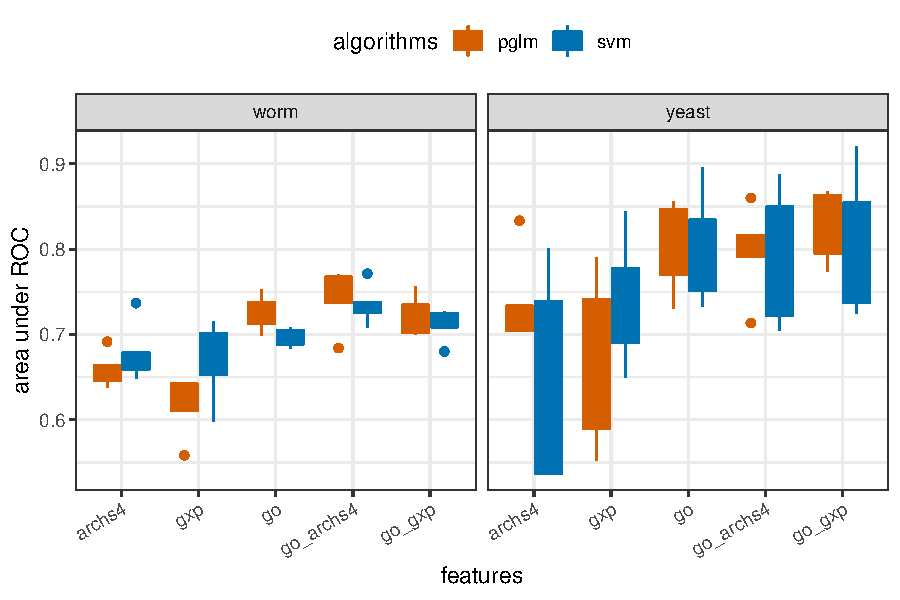
\includegraphics{./auc_svm_pglm.pdf}

\section{Conclusions}

We recommend that future researchers studying aging consider a broad range of algorithms.

\bibliographystyle{plain}
\bibliography{ade}

\end{document}